\documentclass{theozettel}

%%%%%%%%%%%%%%%%%%%%%%%%%%%%%%%%%%%%%%%%%%%%%%%%%%%%%%%%%%%%%%%%%%%%%%%%%%%%%%%%%%%%%%%%%%%%%%%%%%%%%%%%%%%%%%
% page geometry
%%%%%%%%%%%%%%%%%%%%%%%%%%%%%%%%%%%%%%%%%%%%%%%%%%%%%%%%%%%%%%%%%%%%%%%%%%%%%%%%%%%%%%%%%%%%%%%%%%%%%%%%%%%%%%
\geometry{
	left=20mm,
	right=20mm,
	top=25mm,
	bottom=20mm
}
%%%%%%%%%%%%%%%%%%%%%%%%%%%%%%%%%%%%%%%%%%%%%%%%%%%%%%%%%%%%%%%%%%%%%%%%%%%%%%%%%%%%%%%%%%%%%%%%%%%%%%%%%%%%%%

\pgfplotsset{compat=1.16}

%\renewcommand{\phi}{\varphi}

\usepackage{parskip}
\usepackage{dsfont}
\newcommand{\difd}{\text{d}}
\usepackage{titlesec} 
\titleformat{\section}[runin]
{\normalfont\large\bfseries}{\thesubsection}{1em}{}
\titleformat{\subsection}[runin]
  {\normalfont\normalsize\bfseries}{\thesubsubsection}{1em}{}
  

\theoI{5}

\begin{document}
\punkteV{5.1}{5.2}{5.3}{5.4}{5.5}

\section*{Aufgabe 7.1} 

a)

Sei $x(t)$ die Länge des Teils des Seils, das zu dem Zeitpunkt $t$ von der Tischkante hinabhängt. Die Gewichtskraft, die auf dieses Ende wirkt, ist die Kraft, die die Bewegung des Seils beeinflusst, bzw. gleich $m \ddot{x}$. Somit gilt:

$$
\ddot{x} = \frac{F_g(t)}{m} = \frac{\mu g x(t)}{m} = \frac{g}{L} x(t) =: K x(t)
$$

Um diese DGL zu lösen, machen wir den Ansatz $x(t) = e^{ct}$, setzen dies in die DGL ein und bestimmen $c$ durch umformen:

$$
c^{2} e^{ct} = K e^{ct}
$$

$$
c = \pm \sqrt{K}
$$

Somit haben wir zwei spezielle Lösungen der DGL gefunden. Die allgemeine Lösung ergibt sich nun als allgemeine Linearkombination der beiden speziellen Lösungen:

$$
x(t) = A e^{\sqrt{K} t} + B e^{- \sqrt{K} t}
$$

Wir definieren den Zeitpunkt, wann die Kette anfängt sich zu bewegen als $t_0 = 0$.

Nun können wir $A$ und $B$ mithilfe unserer Anfangsbedingungen herausfinden:

\begin{align*}
\dot{x}(0) = 0 &= \sqrt{K} (A e^{\sqrt{K} 0} - B e^{- \sqrt{K} 0}) \\
&= A - B \\
A &= B
\end{align*}


\begin{align*}
x(0) = x_0 &= A e^{\sqrt{K} 0} + B e^{- \sqrt{K} 0} \\
&= A + B \\
A &= \frac{x_0}{2} \\
B &= \frac{x_0}{2}
\end{align*}

Somit ergibt sich:

$$
x(t) = x_0 \cosh(\sqrt{K} t) = x_0 \cosh(\sqrt{\frac{g}{L}} t)
$$

Die Gleichung gilt offensichtlich nur bis zum Zeitpunkt $T$.


b)

Die Anfangsgeschwindigkeit des freien Falls ist offensichtlich $\dot{x}(T)$. Hierfür wird zunächst $T$ berechnet:

$$
x(T) =  x_0 \cosh(\sqrt{\frac{g}{L}} T) = L
$$

$$
T = \text{arccosh}(\frac{L}{g}) \sqrt{\frac{L}{g}}
$$

$\dot{x}(T)$ ergibt somit:

$$
\dot{x}(T) = x_0 \sqrt{\frac{g}{L}} \sinh(\sqrt{\frac{g}{L}} T) = x_0 \sqrt{\frac{g}{L}} \sqrt{(\cosh( \sqrt{\frac{g}{L}} \sqrt{\frac{L}{g}} \text{arccosh}(\frac{L}{x_0}))^{2} - 1)} = \sqrt{\frac{g}{L} (L^{2} - x_0^{2})}
$$

c) 
%Bei dieser Teilaufgabe bin ich mir nicht sicher ob ich es richtig habe (bzw auch nicht sicher, ob ich es überhaupt richtig verstanden habe.)

In diesem Fall gibt es noch die Gleitreibung, die der Gewichtskraft entgegen wirkt. Somit verändert sich die DGL wie folgt:

$$
\ddot{x} = \frac{F_g(t) - F_{Gl}(t)}{m} = \frac{\mu g x(t) - \eta (L-x(t))}{m} = \frac{\mu g + \eta}{\mu L} x - \frac{\eta L}{m} =: K' x - \frac{\eta}{\mu}
$$

Der homogene Teil der DGL (ohne das $\frac{\eta}{\mu}$) lässt sich wie in Aufgabenteil a) lösen. Da der inhomogene Teil eine Konstante, bzw. unabhängig von $t$ ist, kann diese inhomogene DGL durch das addieren einer Konstanten $C$ zu der Lösung der homogenen DGL $x_{hom}$ gelößt werden, da hierdurch die Ableitungen von $x$ unverändert bleiben und die Konstante den inhomogenen Term ausgleichen kann:

$$
\ddot{x_{hom}} = K' x_{hom} = \ddot{x} = K' x - \frac{\eta}{\mu} = K' (x_{hom} + C) - \frac{\eta}{\mu}
$$

Das $C$ muss somit Folgendes sein:

$$
C = \frac{\eta}{\mu K'} =  \frac{\eta L}{\mu g + \eta}
$$

Nun kann man können wir die allgemeine Lösung der homogenen Gleichung einsetzen und mit denn Anfangsbedingungen wie in Aufgabenteil a) die Konstanten herausfinden:

$$
x(0) = A e^{-\sqrt{K'} 0} + B e^{\sqrt{K'} 0} + C = x_0
$$

Also:

$$
A + B = x_0 - C
$$

$$
\dot{x}(0) = -\sqrt{K'} A e^{-\sqrt{K'} 0} + \sqrt{K'}B e^{\sqrt{K'} 0} = 0
$$

Somit gilt $A = B$. Zusammen ergeben die Bedingungen:

$$
A = B = \frac{x_0 - C}{2} = \frac{x_0 - \frac{\eta L}{\mu g + \eta}}{2}
$$

Insgesamt gilt also:

$$
x(t) = (x_0 - \frac{\eta L}{\mu g + \eta}) \cosh(\sqrt{\frac{\mu g + \eta}{\mu L}} t ) + \frac{\eta L}{\mu g + \eta}
$$


\section*{Aufgabe 7.2} 


Einfach ausrechnen:

$$
x(0) = x_0 = a e^{- \gamma 0} + b 0 e^{- \gamma 0} = a
$$

Also gilt $a = x_0$.

$$
\dot{x}(0) = 0 = - \gamma a e^{- \gamma 0} + (b e^{- \gamma 0} - \gamma b 0 e^{- \gamma 0}) = b - \gamma a
$$

Somit gilt $b = \gamma a = \gamma x_0$.



\section*{Aufgabe 7.3} 
Bestimmen Sie die allgemeinen rellen Lösungen für die Differentialgleichungen
\subsection*{a)} $\ddot{x}-5\dot{x}+6x=0$
\begin{align*}
\ddot{x}-5\dot{x}+6x&=0\\
\Rightarrow\lambda^2-5\lambda+6&=0\\
\Leftrightarrow\left(\lambda-2\right)\cdot\left(\lambda-3\right)&=0\\
\Rightarrow\lambda_1=2 \ ;& \ \lambda_2=3\\
\Rightarrow x&=c_1e^{2t}+c_2e^{3t}
\end{align*}
\subsection*{b)}$\dddot{x}+\ddot{x}+4\dot{x}+4x=0$
\begin{align*}
\dddot{x}+\ddot{x}+4\dot{x}+4x&=0\\
\Rightarrow \lambda^3+\lambda^2+4\lambda+4&=0\\
\Leftrightarrow \lambda^2\left(\lambda+1\right)+4\left(\lambda+1\right)&=0\\
\Leftrightarrow\left(\lambda^2+4\right)\left(\lambda+1\right)&=0\\
\Rightarrow \lambda_{1;2}=0\pm 2i \ &; \ \lambda_3=-1\\
\Rightarrow x&=ae^{-t}+b\sin\left(2t\right)+c\cos\left(2t\right)
\end{align*}
\subsection*{c)}$\ddot{x}+6\dot{x}+25x=0$; $x\left(0\right)=5, \ \dot{x}\left(0\right)=-3$
\begin{align*}
\ddot{x}+6\dot{x}+25x&=0\\
\Rightarrow \lambda^2+6\lambda +25&=0\\
\Rightarrow\lambda_{1;2}=\frac{-6\pm\sqrt{6^2-4\cdot 25}}{2}&=-3\pm 4i\\
\Rightarrow x&=e^{-3t}\left(c_1\sin\left(4t\right)+c_2\cos\left(4t\right)\right)\\
\end{align*}
Anfangsbed. einsetzen:
\begin{align*}
x\left(0\right)=5&=e^{-3\cdot 0}\left(c_1\sin\left(4\cdot 0\right)+c_2\cos\left(4\cdot 0\right)\right)\\
5&=c_2\\\\
\dot{x}\left(0\right)=-3&=-3e^{-3\cdot 0}\left(c_1\sin\left(4\cdot 0\right)+5\cos\left(4\cdot 0\right)\right)+e{-3\cdot 0}\left(4c_1\cos\left(4\cdot 0\right)-20\sin\left(4\cdot 0\right)\right)\\
-3&=-15+4c_1\\
c_1&=3\\\\
\Rightarrow x&=e^{-3t}\left(3\sin\left(4t\right)+5\cos\left(4t\right)\right)
\end{align*}
\section*{Aufgabe 7.4} 
\subsection*{a)}Wie in der Vorlesung besprochen, werden Drehungen durch orthogonale Matrizen beschrieben. Die Wirkung auf Vektoren ist $\vec{r}\mapsto\vec{r}'=A\vec{r}$. Geben Sie die Matrix an, welche eine Drehung in der $x$-$y$-Ebene um den Winkel $\varphi$ beschreibt. Wie lautet dann die Matrix $B$, die diese Drehung wieder rückgängig macht? Berechnen Sie die Determinanten von $A$ und $B$.\\\\
Da wir die Vektoren mit dieser Matrix nur drehen wollen, bleiben die tatsächlichen Längen der Vektoren gleich. Somit reicht es, wenn wir die Einheitsvektoren drehen. Nach der Drehung haben diese immer noch die gleiche Länge, jedoch eine andere Ausrichtung.\\
Da wir in der $x$-$y$-Achse drehen, können wir die Drehung in diesem Untervektorraum vollführen. Da dort die $z$-Komponente nicht entscheidend ist, muss diese bei einer späteren Matrixmultiplikation wegfallen:
\begin{align*}
\mqty(a_{11} & a_{12} & a_{13}\\a_{21} &a_{22} & a_{23}\\a_{31} &a_{32} & a_{33})\cdot\mqty(x\\y\\z)&=\mqty(a_{11}x+a_{12}y+a_{13}z\\a_{21}x+a_{22}y+a_{23}z\\a_{31}x+a_{32}y+a_{33}z)\\
\Rightarrow a_{13}=a_{23}=a_{31}&=a_{32}=0\ ; \ a_{33}=1\\\\
\Rightarrow A&=\mqty(a_{11} & a_{12} & 0\\a_{21} &a_{22} & 0\\0 & 0 & 1)
\end{align*}
Diese Form wurde auch im Hinweis gegeben.\\
Betrachten wir nun den $\mathbb{R}^2$ der $x$-$y$-Ebene.
\begin{center}
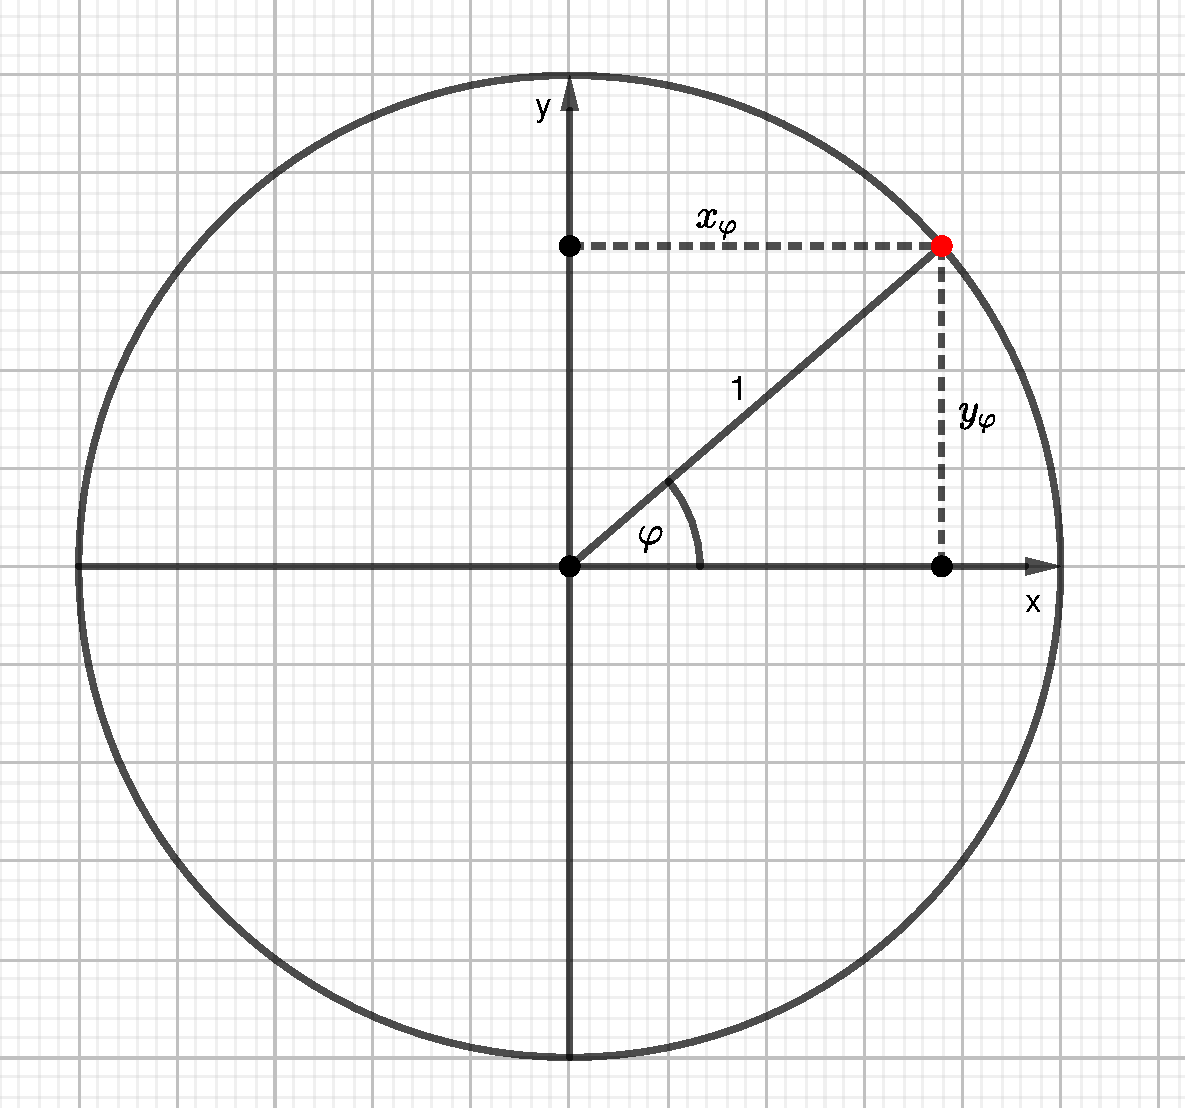
\includegraphics[scale=0.4]{Theo07-4a)_1.pdf}
\end{center}
Um die Drehung des Einheitsvektors der $x$-Achse zu beschreiben reicht:
\begin{align*}
\mqty(a_{11} & a_{12}\\ a_{21} &a_{22})\mqty(1 \\ 0)=\mqty(a_{11}\\ a_{21})
\end{align*}
Die lässt sich einfach per Trigonometrie lösen:
\begin{align*}
\mqty(\cos\left(\varphi\right) & a_{12}\\ \sin\left(\varphi\right) &a_{22})\mqty(1 \\ 0)=\mqty(\cos\left(\varphi\right)\\\sin\left(\varphi\right))
\end{align*}
Nun muss aber auch der Einheitsvektor der $y$-Achse gedreht werden:
\begin{center}
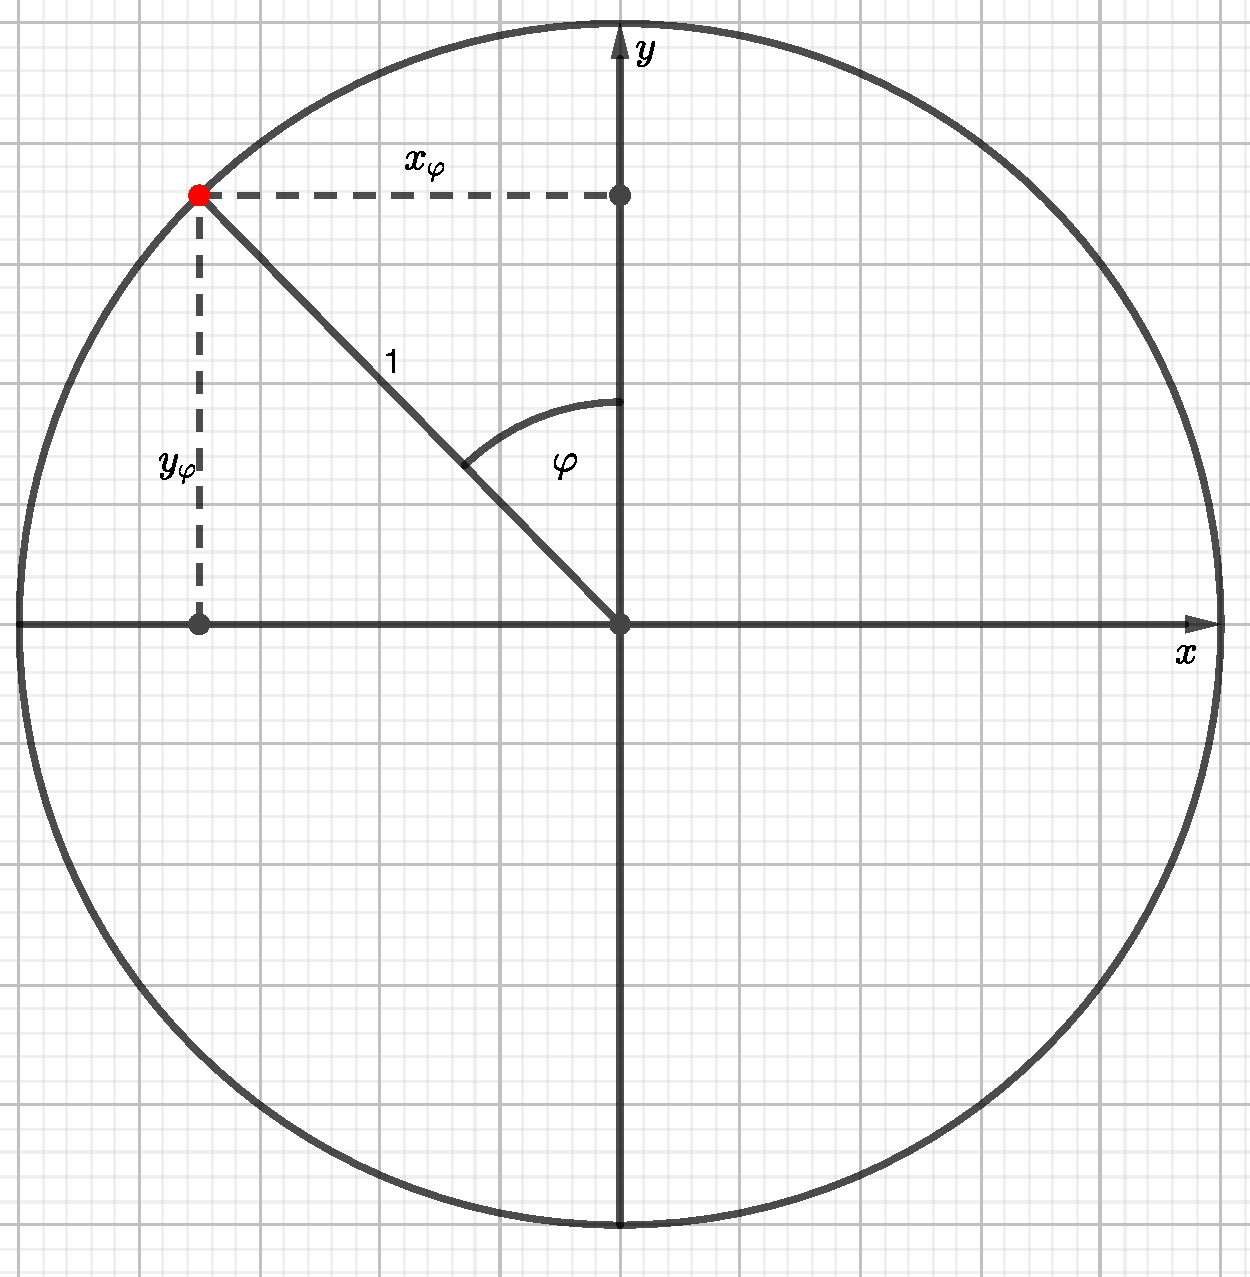
\includegraphics[scale=0.4]{Theo07-4a)_2.pdf}
\end{center}
Um die Drehung des Einheitsvektors der $y$-Achse zu beschreiben reicht:
\begin{align*}
\mqty(a_{11} & a_{12}\\ a_{21} &a_{22})\mqty(0 \\ 1)=\mqty(a_{12}\\ a_{22})
\end{align*}
Die lässt sich einfach per Trigonometrie lösen:
\begin{align*}
\mqty(\cos\left(\varphi\right) & -\sin\left(\varphi\right)\\ \sin\left(\varphi\right) &\cos\left(\varphi\right))\mqty(0 \\ 1)=\mqty(-\sin\left(\varphi\right)\\\cos\left(\varphi\right))
\end{align*}
Nun können wir die Untermatrix einfach in $A$ wieder einsetzen, dies ergibt:
\begin{align*}
A=\mqty(\cos\left(\varphi\right) & -\sin\left(\varphi\right) & 0 \\ \sin\left(\varphi\right) & \cos\left(\varphi\right) & 0\\ 0&0&1)
\end{align*}
Um den Vektor wieder zurückzudrehen, reicht es, ihn einfach um den im Betrag gleichen Winkel in die entgegengesetzte Richtung zu drehen.\\
Somit ist $B\left(\varphi\right)=A\left(-\varphi\right)$:
\begin{align*}
B=\mqty(\cos\left(-\varphi\right) & -\sin\left(-\varphi\right) & 0 \\ \sin\left(-\varphi\right) & \cos\left(-\varphi\right) & 0\\ 0&0&1)=\mqty(\cos\left(\varphi\right) & \sin\left(\varphi\right) & 0 \\ -\sin\left(\varphi\right) & \cos\left(\varphi\right) & 0\\ 0&0&1)
\end{align*}
Die Determinanten von $A$ und $B$ sind gleich, denn:
\begin{align*}
\det\left(A\right)=\cos\left(\varphi\right)^2-\left(-sin\left(\varphi\right)^2\right)&=1\\
\det\left(B\right)=\cos\left(\varphi\right)^2-\left(-sin\left(\varphi\right)^2\right)&=1
\end{align*}
\subsection*{b)}Wie sieht die entsprechende Drehmatrix für eine Drehung in der $x$-$z$-Ebene aus?\\
Wie in \textbf{a)} können wir eine Achse vernachlässigen, in diesem Fall die $y$-Achse.
\begin{align*}
\mqty(a_{11} & a_{12} & a_{13}\\a_{21} &a_{22} & a_{23}\\a_{31} &a_{32} & a_{33})\cdot\mqty(x\\y\\z)&=\mqty(a_{11}x+a_{12}y+a_{13}z\\a_{21}x+a_{22}y+a_{23}z\\a_{31}x+a_{32}y+a_{33}z)\\
\Rightarrow a_{12}=a_{21}=a_{23}&=a_{32}=0\ ; \ a_{22}=1\\\\
\Rightarrow A&=\mqty(a_{11} & 0 & a_{13} \\ 0 &1 & 0\\a_{31} & 0 & a_{33})
\end{align*}
Betrachten wir diesmal die $x$-$z$-Ebene:
\begin{center}
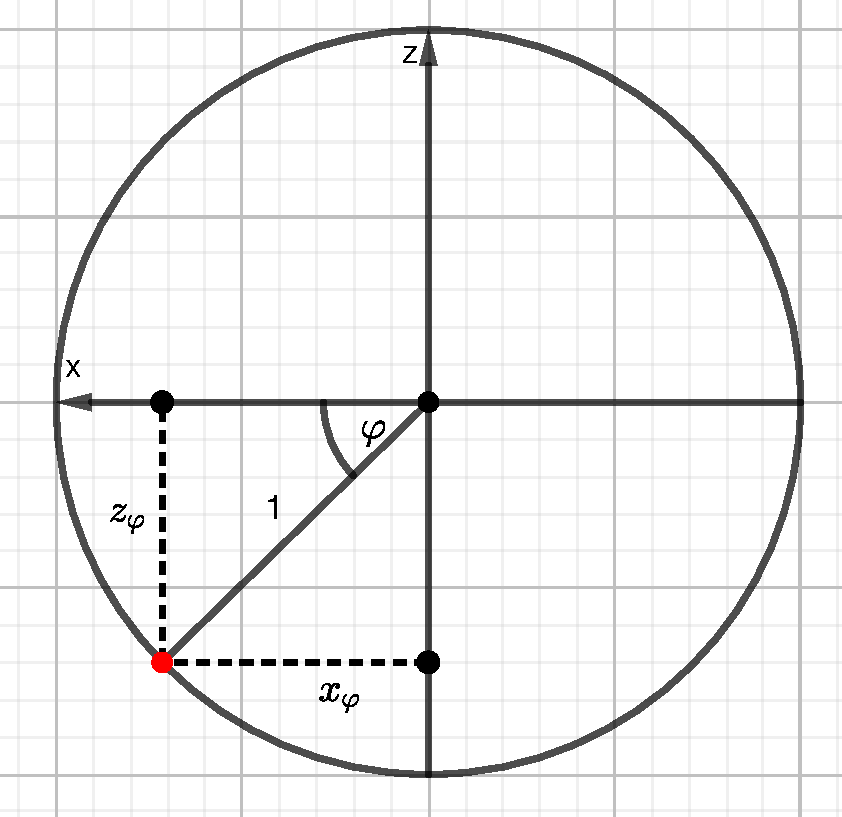
\includegraphics[scale=0.4]{Theo07-4b)_1.pdf}
\end{center}
Um die Drehung des Einheitsvektors der $x$-Achse zu beschreiben reicht:
\begin{align*}
\mqty(a_{11} & a_{13}\\ a_{31} &a_{33})\mqty(1 \\ 0)=\mqty(a_{11}\\ a_{31})
\end{align*}
Die lässt sich einfach per Trigonometrie lösen:
\begin{align*}
\mqty(\cos\left(\varphi\right) & a_{13}\\ -\sin\left(\varphi\right) &a_{33})\mqty(1 \\ 0)=\mqty(\cos\left(\varphi\right)\\-\sin\left(\varphi\right))
\end{align*}
Das $-\sin\left(\varphi\right)$ kommt durch die Richtung des $z$-Einheitsvektors.
Nun muss aber auch der Einheitsvektor der $z$-Achse gedreht werden:
\begin{center}
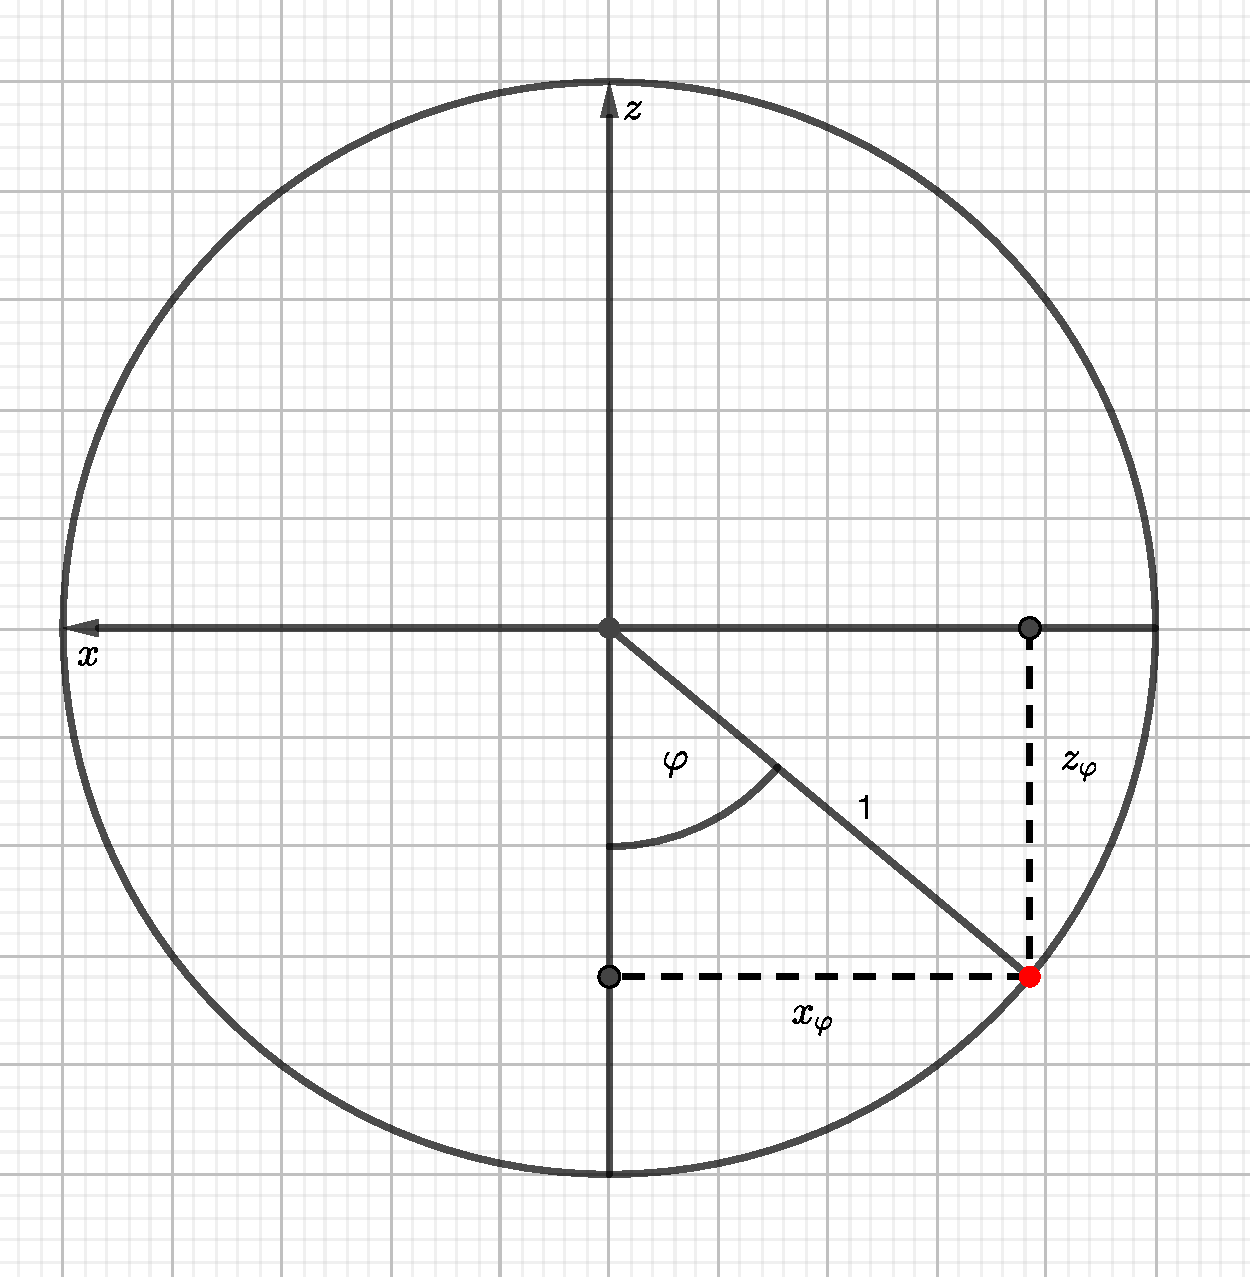
\includegraphics[scale=0.4]{Theo07-4b)_2.pdf}
\end{center}
Um die Drehung des Einheitsvektors der $y$-Achse zu beschreiben reicht:
\begin{align*}
\mqty(a_{11} & a_{13}\\ a_{31} &a_{33})\mqty(0 \\ 1)=\mqty(a_{13}\\ a_{33})
\end{align*}
Die lässt sich einfach per Trigonometrie lösen:
\begin{align*}
\mqty(\cos\left(\varphi\right) & \sin\left(\varphi\right)\\ -\sin\left(\varphi\right) &\cos\left(\varphi\right))\mqty(0 \\ 1)=\mqty(\sin\left(\varphi\right)\\\cos\left(\varphi\right))
\end{align*}
Nun können wir die Untermatrix einfach in $A$ wieder einsetzen, dies ergibt:
\begin{align*}
A=\mqty(\cos\left(\varphi\right)&0&\sin\left(\varphi\right)\\0&1&0\\-\sin\left(\varphi\right)&0&\cos\left(\varphi\right))
\end{align*}
\section*{Aufgabe 7.5} 







\end{document}
